% command to make sure colorboxes don't create whitespace between code lines
\fboxsep=.6pt

% default settings for listings
\lstset{style=python, basicstyle=\scriptsize\ttfamily}

\begin{frame}
    \centering
    \begin{figure}[H]
        \includegraphics[keepaspectratio, width=0.7\paperwidth, height=\paperheight]{\thelogo}
    \end{figure}
    Informatik: Programmieren\\
    \emoji{right-arrow-curving-up} Kapitel 4 (Teil 3): \textbf{Konditionale Schleifen-Abbrüche mit \lstinline[basicstyle=\ttfamily]|while| und \lstinline[basicstyle=\ttfamily]|break|}
\end{frame}

\begin{frame}[fragile]{Spirale: Abbruchkondition?}
    \begin{columns}
        \begin{column}{.7\textwidth}
            \begin{lstlisting}
import turtle as t

def spirale(seite, add, max_seite):
    for _ in range(?):
        t.fd(seite)
        t.rt(90)
        seite+=add

spirale(10, 10, 100)
\end{lstlisting}
            Wie viele Male muss das \lstinline|for _ in range(?)| ausgeführt werden?
            \[\floor{\frac{\text{\texttt{maxseite - seite}}}{\text{\texttt{add}}}} + 1\]
            Es geht auch einfacher$\ldots$
        \end{column}

        \begin{column}{.3\textwidth}
            \begin{figure}
                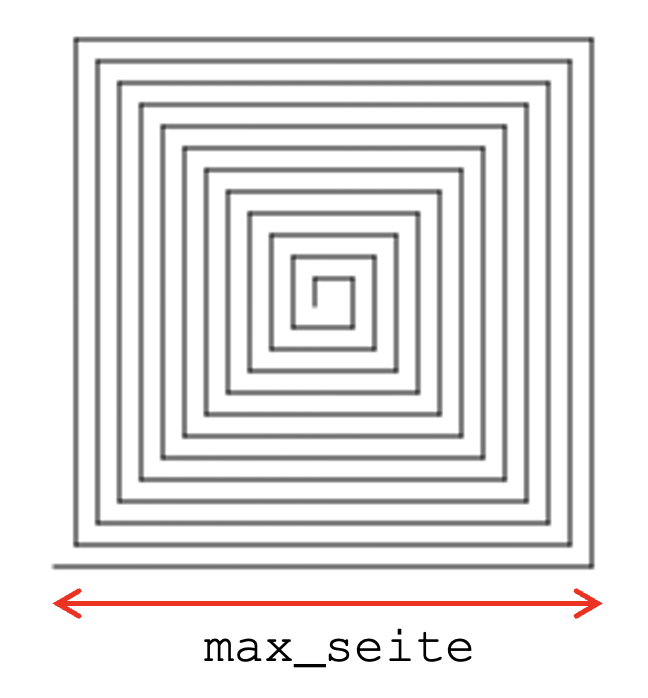
\includegraphics[width=\linewidth]{GrundlagenInfo/00_Programmieren/Figures/spirale_while}
            \end{figure}
        \end{column}
    \end{columns}
\end{frame}

\begin{frame}[fragile]{Spirale: Flussgesteuerter Abbruch (\lstinline[basicstyle=\ttfamily]|break|)}
    \begin{columns}
        \begin{column}{.7\textwidth}
            \begin{lstlisting}[escapechar=!]
import turtle as t

def spirale(seite, add, max_seite):
    while True:!\tikzmark{repeatFrom}!                            !\tikzmark{repeat}!
    	if seite > max_seite:
    	    break!\tikzmark{breakFrom}!                       !\tikzmark{break}!
        t.fd(seite)
        t.rt(90)
        seite+=add

spirale(10, 10, 100)
\end{lstlisting}
        \end{column}
        \begin{column}{.3\textwidth}
            \begin{figure}
                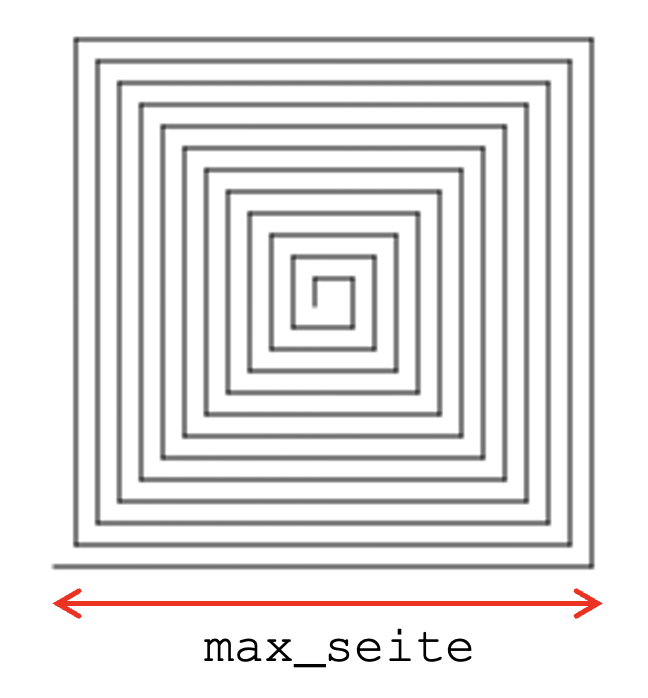
\includegraphics[width=\linewidth]{GrundlagenInfo/00_Programmieren/Figures/spirale_while}
            \end{figure}
        \end{column}
    \end{columns}

    \begin{tikzpicture}[overlay, remember picture,
            every node/.style={draw=red!50,fill=red!50!white,text=black,rounded corners}]
        \drawArrow{repeatFrom}{repeat}{\footnotesize Unendliche Schleife}{CarnationPink};
        \drawArrow{breakFrom}{break}{\footnotesize Schleifenabbruch}{CarnationPink};
    \end{tikzpicture}

\end{frame}

\begin{frame}[fragile]{Fuss- und kopfgesteuerte Schleifen}
    \begin{columns}
        \begin{column}{.47\textwidth}
            \begin{lstlisting}[escapechar=!,basicstyle=\footnotesize\ttfamily]
import turtle as t

def spirale(seite, add, maxS):
    while True:            !\tikzmark{fromStart}!
    	if seite > maxS:
    	    break          !\tikzmark{fromEnd}!
        t.fd(seite)
        t.rt(90)
        seite+=add

spirale(10, 10, 100)
\end{lstlisting}
        \end{column}
        \begin{column}{.5\textwidth}
            \begin{lstlisting}[escapechar=!,basicstyle=\footnotesize\ttfamily]
import turtle as t

def spirale(seite, add, maxS):
    !\tikzmark{toStart}!!\tikzmark{toEnd}!while seite > maxS:
        t.fd(seite)
        t.rt(90)
        seite+=add
        
spirale(10, 10, 100)
\end{lstlisting}
        \end{column}
    \end{columns}

    % annotate listings
    \begin{tikzpicture}[overlay, remember picture,
            every edge/.append style = { ->, thick, >=stealth, red!70},
            every node/.style={draw=red!50,fill=red!50!white,text=black,rounded corners}]
        \only<2->{
            \drawBrace{0em}{fromStart}{fromEnd}{}{.5}{}{}
		    \drawBrace{-.5em}{toStart}{toEnd}{}{.5}{mirror}{}
            % arrow pointing from one code to other
            \draw[->, style={thick, >=stealth, red!70}] (fromStartfromEnd-coord-arrow) to (toStarttoEnd-coord-arrow);
        }
    \end{tikzpicture}
\end{frame}

\begin{frame}[fragile]{Wichtige Bemerkungen}
    \begin{itemize}[<+->]
        \item \lstinline|break| bricht nicht aus \lstinline|def| aus, sondern aus der (aktuellen) \lstinline|while True|-Schleife!
        \item Ein \lstinline|while True:| (unendliche Schleife) ohne \lstinline|break| kann zum Absturz des Programms führen \emoji{face-with-spiral-eyes}
        \item Je nachdem kann das auch in einem \lstinline|while| passieren, sofern die Bedingung nach dem \lstinline|while| so geschrieben ist, dass sie immer wahr (\lstinline|True|) ist.
        \item \textbf{Speichern Sie regelmässig Ihre Aufgaben!}
        \item Falls das Programm TigerJython hängenbleibt: Beenden mit \keys{Ctrl+Alt+\backdel} (Windows), bzw. Activity Monitor unter MacOS
    \end{itemize}
\end{frame}

\begin{frame}[fragile]{Aufträge}
    \begin{itemize}
        \item \aufgabebox{Aufgaben 5.22, 5.23}
        %\item \aufgabebox{Aufgaben 4.31}
        %\item \readbox{S.82 (unten) - S.83}
        %\item \readbox{Beispiel 4.8}
        %\item \abgabebox{Aufgaben 4.33 (ohne %Flussdiagramme)}
        %\item \aufgabebox{Aufgaben 4.38-4.41, 4.43-4.45 (ohne Flussdiagramme)}
        %\item \abgabebox{Aufgaben 4.46 (ohne Flussdiagramme)}
    \end{itemize}
\end{frame}
